\chapter{Síťový ovladač}\label{chpt:MatrixEditor}
Pro centrální dálkové ovládání databází spojení na jednotlivých přípravcích v síti byl vytvořen jednoduchý program v jazyce Python. V době odevzdávání této semestrální práce existuje ovladač pouze jako konzolový skript, v plánu je však vytvořit i uživatelsky mnohem přívětivější aplikaci s grafickým rozhraním.

\begin{figure}[h]
    \centering
    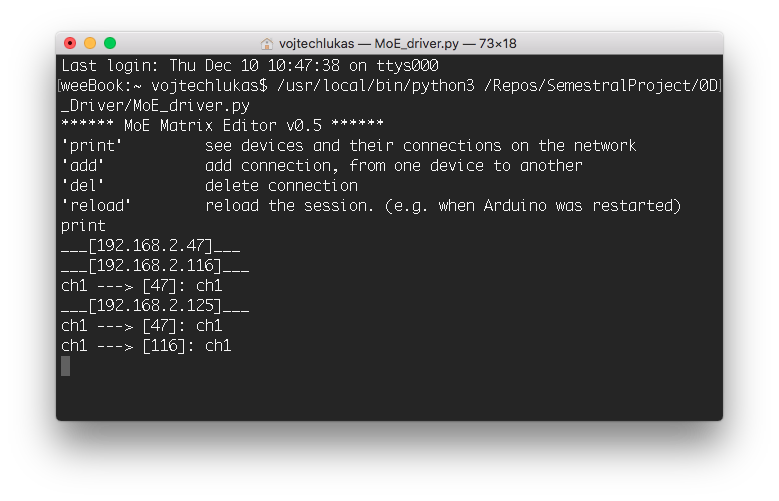
\includegraphics[width=0.7\textwidth]{obrazky/MoE_editor_1.png}
    \caption{Terminálová aplikace \emph{MoE Matrix Editor.}}
    \label{fig:Driver_1}
\end{figure}

Za běhu programu má uživatel na výběr ze čtyř příkazů.
\begin{table}[h]
    \centering
        \begin{tabular}{l p{0.5\textwidth}}
            \texttt{print} & Na konzoli vytiskne všechna zařízení v síti a jejich aktuální spojení. \\
            \texttt{add} & Přidá vybranému zařízení záznam do databáze spojení \texttt{subscriptions}. \\
            \texttt{del} & Vymaže vybranému zařízení záznam z databáze spojení. \\
            \texttt{reload} & Vyžádá si po všech zařízeních na síti aktualizaci jejich databází spojení. \\
        \end{tabular}
\end{table}

Pro pohodlnost je přidáno \uv{makro}, které se spouští zadáním hodnoty \texttt{255} do pole pro cílový kanál zařízení.
